
\documentclass[letterpaper,hide notes,xcolor={table,svgnames},pdftex,10pt]{beamer}
\def\showexamples{t}


%\usepackage[svgnames]{xcolor}

%% Demo talk
%\documentclass[letterpaper,notes=show]{beamer}

\usecolortheme{crane}
\setbeamertemplate{navigation symbols}{}

\usetheme{MyPittsburgh}
%\usetheme{Frankfurt}

%\usepackage{tipa}

\usepackage{hyperref}
\usepackage{graphicx,xspace}
\usepackage[normalem]{ulem}
\usepackage{multicol}

\newcommand\SF[1]{$\bigstar$\footnote{SF: #1}}

\usepackage[default]{sourcesanspro}
\usepackage[T1]{fontenc}

\newcounter{tmpnumSlide}
\newcounter{tmpnumNote}

% old question code
%\newcommand\question[1]{{$\bigstar$ \small \onlySlide{2}{#1}}}
% \newcommand\nquestion[1]{\ifdefined \presentationonly \textcircled{?} \fi \note{\par{\Large \textbf{?}} #1}}
% \newcommand\nanswer[1]{\note{\par{\Large \textbf{A}} #1}}


 \newcommand\mnote[1]{%
   \addtocounter{tmpnumSlide}{1}
   \ifdefined\showcues {~\tiny\fbox{\arabic{tmpnumSlide}}}\fi
   \note{\setlength{\parskip}{1ex}\addtocounter{tmpnumNote}{1}\textbf{\Large \arabic{tmpnumNote}:} {#1\par}}}

\newcommand\mmnote[1]{\note{\setlength{\parskip}{1ex}#1\par}}

%\newcommand\mnote[2][]{\ifdefined\handoutwithnotes {~\tiny\fbox{#1}}\fi
% \note{\setlength{\parskip}{1ex}\textbf{\Large #1:} #2\par}}

%\newcommand\mnote[2][]{{\tiny\fbox{#1}} \note{\setlength{\parskip}{1ex}\textbf{\Large #1:} #2\par}}

\newcommand\mquestion[2]{{~\color{red}\fbox{?}}\note{\setlength{\parskip}{1ex}\par{\Large \textbf{?}} #1} \note{\setlength{\parskip}{1ex}\par{\Large \textbf{A}} #2\par}\ifdefined \presentationonly \pause \fi}

\newcommand\blackboard[1]{%
\ifdefined   \showblackboard
  {#1}
  \else {\begin{center} \fbox{\colorbox{blue!30}{%
         \begin{minipage}{.95\linewidth}%
           \hspace{\stretch{1}} Some space intentionally left blank; done at the blackboard.%
         \end{minipage}}}\end{center}}%
         \fi%
}



%\newcommand\q{\tikz \node[thick,color=black,shape=circle]{?};}
%\newcommand\q{\ifdefined \presentationonly \textcircled{?} \fi}

\usepackage{listings}
\lstset{%
  keywordstyle=\bfseries,
  aboveskip=15pt,
  belowskip=15pt,
  captionpos=b,
  identifierstyle=\ttfamily,
  escapeinside={(*@}{@*)},
  stringstyle=\ttfamiliy,
  frame=lines,
  numbers=left, basicstyle=\scriptsize, numberstyle=\tiny, stepnumber=0, numbersep=2pt}

\usepackage{siunitx}
\newcommand\sius[1]{\num[group-separator = {,}]{#1}\si{\micro\second}}
\newcommand\sims[1]{\num[group-separator = {,}]{#1}\si{\milli\second}}
\newcommand\sins[1]{\num[group-separator = {,}]{#1}\si{\nano\second}}
\sisetup{group-separator = {,}, group-digits = true}

%% -------------------- tikz --------------------
\usepackage{tikz}
\usetikzlibrary{positioning}
\usetikzlibrary{arrows,backgrounds,automata,decorations.shapes,decorations.pathmorphing,decorations.markings,decorations.text}

\tikzstyle{place}=[circle,draw=blue!50,fill=blue!20,thick, inner sep=0pt,minimum size=6mm]
\tikzstyle{transition}=[rectangle,draw=black!50,fill=black!20,thick, inner sep=0pt,minimum size=4mm]

\tikzstyle{block}=[rectangle,draw=black, thick, inner sep=5pt]
\tikzstyle{bullet}=[circle,draw=black, fill=black, thin, inner sep=2pt]

\tikzstyle{pre}=[<-,shorten <=1pt,>=stealth',semithick]
\tikzstyle{post}=[->,shorten >=1pt,>=stealth',semithick]
\tikzstyle{bi}=[<->,shorten >=1pt,shorten <=1pt, >=stealth',semithick]

\tikzstyle{mut}=[-,>=stealth',semithick]

\tikzstyle{treereset}=[dashed,->, shorten >=1pt,>=stealth',thin]

\usepackage{ifmtarg}
\usepackage{xifthen}
\makeatletter
% new counter to now which frame it is within the sequence
\newcounter{multiframecounter}
% initialize buffer for previously used frame title
\gdef\lastframetitle{\textit{undefined}}
% new environment for a multi-frame
\newenvironment{multiframe}[1][]{%
\ifthenelse{\isempty{#1}}{%
% if no frame title was set via optional parameter,
% only increase sequence counter by 1
\addtocounter{multiframecounter}{1}%
}{%
% new frame title has been provided, thus
% reset sequence counter to 1 and buffer frame title for later use
\setcounter{multiframecounter}{1}%
\gdef\lastframetitle{#1}%
}%
% start conventional frame environment and
% automatically set frame title followed by sequence counter
\begin{frame}%
\frametitle{\lastframetitle~{\normalfont(\arabic{multiframecounter})}}%
}{%
\end{frame}%
}
\makeatother

\makeatletter
\newdimen\tu@tmpa%
\newdimen\ydiffl%
\newdimen\xdiffl%
\newcommand\ydiff[2]{%
    \coordinate (tmpnamea) at (#1);%
    \coordinate (tmpnameb) at (#2);%
    \pgfextracty{\tu@tmpa}{\pgfpointanchor{tmpnamea}{center}}%
    \pgfextracty{\ydiffl}{\pgfpointanchor{tmpnameb}{center}}%
    \advance\ydiffl by -\tu@tmpa%
}
\newcommand\xdiff[2]{%
    \coordinate (tmpnamea) at (#1);%
    \coordinate (tmpnameb) at (#2);%
    \pgfextractx{\tu@tmpa}{\pgfpointanchor{tmpnamea}{center}}%
    \pgfextractx{\xdiffl}{\pgfpointanchor{tmpnameb}{center}}%
    \advance\xdiffl by -\tu@tmpa%
}
\makeatother
\newcommand{\copyrightbox}[3][r]{%
\begin{tikzpicture}%
\node[inner sep=0pt,minimum size=2em](ciimage){#2};
\usefont{OT1}{phv}{n}{n}\fontsize{4}{4}\selectfont
\ydiff{ciimage.south}{ciimage.north}
\xdiff{ciimage.west}{ciimage.east}
\ifthenelse{\equal{#1}{r}}{%
\node[inner sep=0pt,right=1ex of ciimage.south east,anchor=north west,rotate=90]%
{\raggedleft\color{black!50}\parbox{\the\ydiffl}{\raggedright{}#3}};%
}{%
\ifthenelse{\equal{#1}{l}}{%
\node[inner sep=0pt,right=1ex of ciimage.south west,anchor=south west,rotate=90]%
{\raggedleft\color{black!50}\parbox{\the\ydiffl}{\raggedright{}#3}};%
}{%
\node[inner sep=0pt,below=1ex of ciimage.south west,anchor=north west]%
{\raggedleft\color{black!50}\parbox{\the\xdiffl}{\raggedright{}#3}};%
}
}
\end{tikzpicture}
}


%% --------------------

%\usepackage[excludeor]{everyhook}
%\PushPreHook{par}{\setbox0=\lastbox\llap{MUH}}\box0}

%\vspace*{\stretch{1}

%\setbox0=\lastbox \llap{\textbullet\enskip}\box0}

\setlength{\parskip}{\fill}

\newcommand\noskips{\setlength{\parskip}{1ex}}
\newcommand\doskips{\setlength{\parskip}{\fill}}

\newcommand\xx{\par\vspace*{\stretch{1}}\par}
\newcommand\xxs{\par\vspace*{2ex}\par}
\newcommand\tuple[1]{\langle #1 \rangle}
\newcommand\code[1]{{\sf \footnotesize #1}}
\newcommand\ex[1]{\uline{Example:} \ifdefined \presentationonly \pause \fi
  \ifdefined\showexamples#1\xspace\else{\uline{\hspace*{2cm}}}\fi}

\newcommand\ceil[1]{\lceil #1 \rceil}


\AtBeginSection[]
{
   \begin{frame}
       \frametitle{Outline}
       \tableofcontents[currentsection]
   \end{frame}
}



\pgfdeclarelayer{edgelayer}
\pgfdeclarelayer{nodelayer}
\pgfsetlayers{edgelayer,nodelayer,main}

\tikzstyle{none}=[inner sep=0pt]
\tikzstyle{rn}=[circle,fill=Red,draw=Black,line width=0.8 pt]
\tikzstyle{gn}=[circle,fill=Lime,draw=Black,line width=0.8 pt]
\tikzstyle{yn}=[circle,fill=Yellow,draw=Black,line width=0.8 pt]
\tikzstyle{empty}=[circle,fill=White,draw=Black]
\tikzstyle{bw} = [rectangle, draw, fill=blue!20, 
    text width=4em, text centered, rounded corners, minimum height=2em]
    
    \newcommand{\CcNote}[1]{% longname
	This work is licensed under the \textit{Creative Commons #1 3.0 License}.%
}
\newcommand{\CcImageBy}[1]{%
	\includegraphics[scale=#1]{creative_commons/cc_by_30.pdf}%
}
\newcommand{\CcImageSa}[1]{%
	\includegraphics[scale=#1]{creative_commons/cc_sa_30.pdf}%
}
\newcommand{\CcImageNc}[1]{%
	\includegraphics[scale=#1]{creative_commons/cc_nc_30.pdf}%
}
\newcommand{\CcGroupBySa}[2]{% zoom, gap
	\CcImageBy{#1}\hspace*{#2}\CcImageNc{#1}\hspace*{#2}\CcImageSa{#1}%
}
\newcommand{\CcLongnameByNcSa}{Attribution-NonCommercial-ShareAlike}

\newenvironment{changemargin}[1]{% 
  \begin{list}{}{% 
    \setlength{\topsep}{0pt}% 
    \setlength{\leftmargin}{#1}% 
    \setlength{\rightmargin}{1em}
    \setlength{\listparindent}{\parindent}% 
    \setlength{\itemindent}{\parindent}% 
    \setlength{\parsep}{\parskip}% 
  }% 
  \item[]}{\end{list}} 




\title{Lecture 2 --- Constitution and Charter }

\author{Douglas W. Harder \& Jeff Zarnett \\ \small \texttt{dwharder@uwaterloo.ca}~\texttt{jzarnett@uwaterloo.ca}}
\institute{Department of Electrical and Computer Engineering \\
  University of Waterloo}
\date{\today}


\begin{document}

\begin{frame}
  \titlepage

\begin{center}
  \small{Acknowledgments: Douglas Harder~\cite{dwh}, Julie Vale~\cite{jv}}
  \end{center}
\end{frame}


\part{The Canadian Constitution}
\begin{frame}
\partpage

\end{frame}

\begin{frame}
\frametitle{The Canadian Constitution}

The Constitution Acts of 1867 and 1982 are documents providing the legal foundation for the country of Canada.

The original act of 1867 was called the British North America Act.

The constitutional documents were patriated in 1982. 

\end{frame}



\begin{frame}
\frametitle{The Canadian Constitution}

\begin{center}
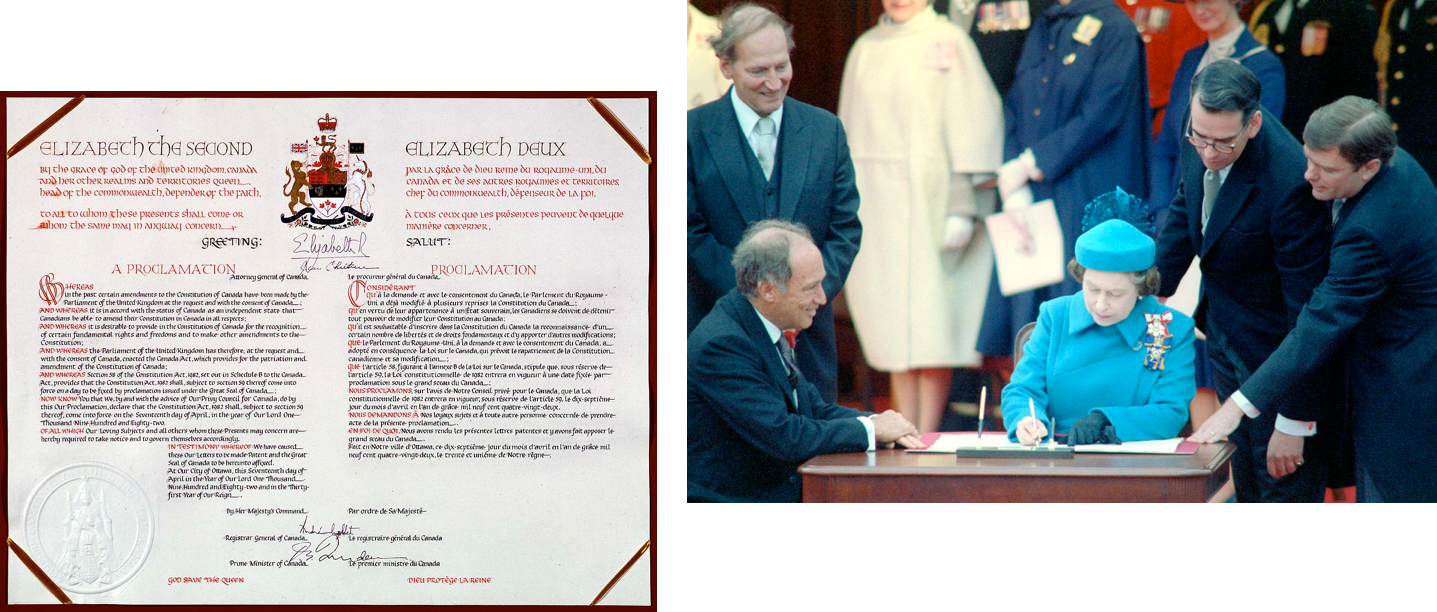
\includegraphics[width=\textwidth]{images/canadian-constitution.png}
\end{center}

\end{frame}



\begin{frame}
\frametitle{The Constitution Act, 1867}

The Constitution Act, 1867 defines:

\begin{itemize}
\item Canada as a union of provinces
\item The executive power of the government
\item The legislative powers of the Senate and House of Commons
\item The executive and legislative powers of the provinces
\end{itemize}


\end{frame}



\begin{frame}
\frametitle{The Constitution Act, 1867}

These define the composition and running of the government and the various legislative bodies, e.g.

\textbf{Duration of House of Commons}\\
\quad \textbf{50.}	Every House of Commons shall continue for Five Years from 
	the Day of the Return of the Writs for choosing the House 
	(subject to be sooner dissolved by the Governor General), and 
	no longer.

\end{frame}



\begin{frame}
\frametitle{Taxation and Expenditures}
The constitution requires that any public spending or tax must come from the House of Commons.

No other entity can make the government spend money or introduce/raise taxes.

\quad \textbf{53.}	Bills for appropriating any Part of the Public
		Revenue, or for imposing any Tax or Impost, shall 
		originate in the House of Commons.

\end{frame}



\begin{frame}
\frametitle{Distribution of Powers}
Canada is officially a federation of provinces.

The head of state is Her Majesty, Queen Elizabeth II, who is represented by the Governor General.

Note that Queen Elizabeth II is Queen of Canada (in addition to being Queen of the United Kingdom. The titles are separate, but held by the same person).

The head of state for each province is also the Queen, represented by the Lieutenant Governors.

There is no hierarchy; all are direct representatives of the Queen.

\end{frame}



\begin{frame}
\frametitle{Levels of Government}

The constitution allows a federal government and a provincial government.

What about municipalities/regions, e.g., City of Toronto or Region of Waterloo?

Authority is delegated to these entities from the province. 

They have only the powers and authority the province chooses to grant.

\end{frame}



\begin{frame}
\frametitle{Conflicts Between Levels}

Provincial legislatures and the federal parliament can both pass laws.

Sometimes there is a conflict.

What happens if the federal government passes a law related to engineering, and it is in conflict with some part of the Professional Engineers Act in Ontario?

Which takes precedence and why?

\end{frame}



\begin{frame}
\frametitle{Distribution of Powers}

The constitution designates certain matters as federal; others as provincial. 

Federal powers: national defence, foreign affairs, banking, criminal law...

Provincial: health care, prisons, education...

Some are shared: agriculture \& immigration...

\end{frame}



\begin{frame}
\frametitle{Stick to What You're Good At}
If a law relates to matters where another legislature has jurisdiction, this law may be challenged in court.

The court may find that the law (or part of it) to be \alert{ultra vires}.

\textit{Ultra vires}: beyond the powers.

\end{frame}



\begin{frame}
\frametitle{\textit{Ultra Vires}}

Recently there was an attempt to create a national securities regulator.

The federal government wished to unify the regulatory regimes in the various provinces which have similar but not identical rules.

The question was: is the proposed act within the legislative authority of the Parliament of Canada?

The Supreme Court of Canada (SCC) ruled that the matter was not.

\end{frame}



\begin{frame}
\frametitle{\textit{Ultra Vires}}
Included in the decision of the Supreme Court was:
\begin{quote}
   ... Canada's problem is that the proposed Act reflects an attempt that goes well beyond these matters of undoubted national interest and concern and reaches down into the detailed regulation of all aspects of securities. In this respect, the proposed Act is unlike federal competition legislation, which has been held to fall under s. 91(2)\footnote{The Regulation of Trade and Commerce} of the Constitution Act, 1867. It would regulate all aspects of contracts for securities within the provinces, including all aspects of public protection and professional competence within the provinces. Competition law, by contrast, regulates only anti-competitive contracts and conduct -- a particular aspect of economic activity that falls squarely within the federal domain. In short, the proposed federal Act overreaches the legislative interest of the federal government.
\end{quote}
\end{frame}



\begin{frame}
\frametitle{The Courts}

The subject of the Supreme Court has already appeared.

As the name suggests, it is the highest court in the land.

We will return to the subject of the court's shortly.

\end{frame}



\begin{frame}
\frametitle{Changing the Constitution}
Prior to 1982, the Constitution Act, 1867, was the British North America Act, 1867 and was an act of the British parliament.

Thus, a simple majority of the British House of Commons and House of Lords was adequate to change it.

The act had been amended between 1867 and 1982, but only with the consent of Canada's representatives.

The Canada Act, 1982, was passed in the British parliament to grant Canada its own constitution.

\end{frame}



\begin{frame}
\frametitle{Amendments}

As the constitution is now a Canadian Act, it must include in it a formula for constitutional changes.

General procedure for amending Constitution of Canada:

\textbf{38.} (1)	An amendment to the Constitution of Canada may be 
		made by proclamation issued by the Governor General 
		under the Great Seal of Canada where so authorized by\\
\quad			(a)	resolutions of the Senate and House of Commons; and\\
\quad		(b)	resolutions of the legislative assemblies of \textbf{at least
			two-thirds of the provinces} that have, in the 
			aggregate, according to the then latest general census,
			\textbf{at least fifty per cent of the population} of all the 
			provinces.

Do not underestimate how difficult this makes amending the constitution...

\end{frame}

\part{The Charter of Rights and Freedoms}



\begin{frame}
\partpage
\end{frame}



\begin{frame}
\frametitle{\textit{Vis et Voluntas}}

In ancient times, monarchs of England ruled on the principle of \textit{vis et voluntas}, or ``Force and Will''.

They made arbitrary decisions and operated on the principle that the King was above the law.\footnote{``Well, when the president does it, that means it is not illegal.
'' - Richard Nixon}.

In theory, a King was supposed to rule justly and fairly, following both custom and law, and with the advice of others.

But there were no rules about what happened if the King did not.

Henry I\footnote{One of the sons of William the Conqueror} decided to voluntarily limit his powers with a Charter of Liberties.

\end{frame}



\begin{frame}
\frametitle{\textit{Magna Carta}}

By 1215 the situation in England was dire for the monarchy.

The taxes and arbitrary rule of King John caused barons (lower level nobility) to rebel against his rule.

He had also lost Normandy to the French and felt compelled to pledge himself as a crusader to win the favour of the Pope.

His barons forced King John to sign the \textit{Magna Carta} - Great Charter - at Runnymede in 1215.

King John immediately wanted to take it back, so he asked the Pope to officially annul it. 

Pope Innocent III did so, and this sparked more war (whoops).

\end{frame}



\begin{frame}
\frametitle{\textit{Magna Carta}}

In spite of this, the principles of it remained in force.

The charter was central to the establishment of parliament.

It also contained a clause enshrining the right to Due Process.

\textbf{29.} NO Freeman shall be taken or imprisoned,
	or be disseised of his Freehold, or
	Liberties, or free Customs, or be outlawed,
	or exiled, or any other wise destroyed; nor 
	will We not pass upon him, nor condemn 
	him, but by lawful judgment of his Peers,
	or by the Law of the land. We will sell to no
	man, we will not deny or defer to any man 
	either Justice or Right.

\end{frame}



\begin{frame}
\frametitle{U-S-A!}

Another step in liberty came with the founding of the United States of America.

The constitution as originally drafted had no statement of rights, so the first ten amendments were introduced and passed and were known as the Bill of Rights.

From watching US TV shows or news you may know more about these rights than the ones you have in Canada...

\end{frame}



\begin{frame}
\frametitle{Canadian Bill of Rights}

In 1947, Saskatchewan introduced a provincial Bill of Rights.

In 1960, the federal government introduced the Canadian Bill of Rights.

It protected numerous rights\footnote{\url{https://en.wikipedia.org/wiki/Canadian\_Bill\_of\_Rights}}:

\begin{itemize}
\item Freedom of speech in Canada and freedom of religion in Canada
\item Equality rights
\item The right to life, liberty and security of the person, rights to fundamental justice
\item The right to enjoyment of property, which is not enshrined in the Charter
\item The right to counsel
\end{itemize}

\end{frame}



\begin{frame}
\frametitle{Canadian Bill of Rights}

\begin{center}
	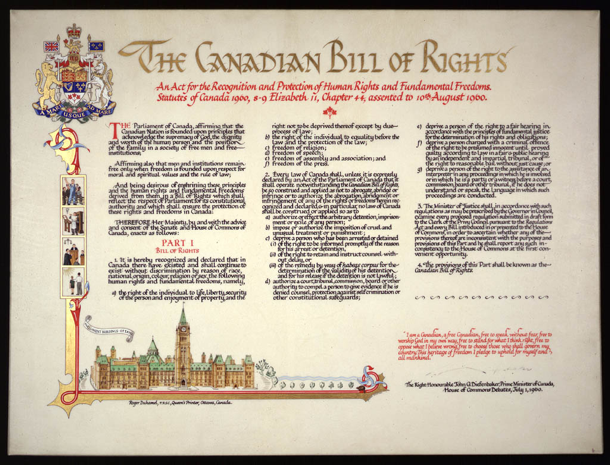
\includegraphics{images/canadian-bill-of-rights.png}
\end{center}

\end{frame}



\begin{frame}
\frametitle{The Charter of Rights and Freedoms}
This was merely a federal act and not part of the constitution.

A great deal of debate arose about whether it was binding on other levels of government or even future governments.

These weaknesses plus the success of the US Bill of Rights led to the Charter as part of the Constitution Act 1982.

\end{frame}



\begin{frame}
\frametitle{The Charter of Rights and Freedoms}

\begin{center}
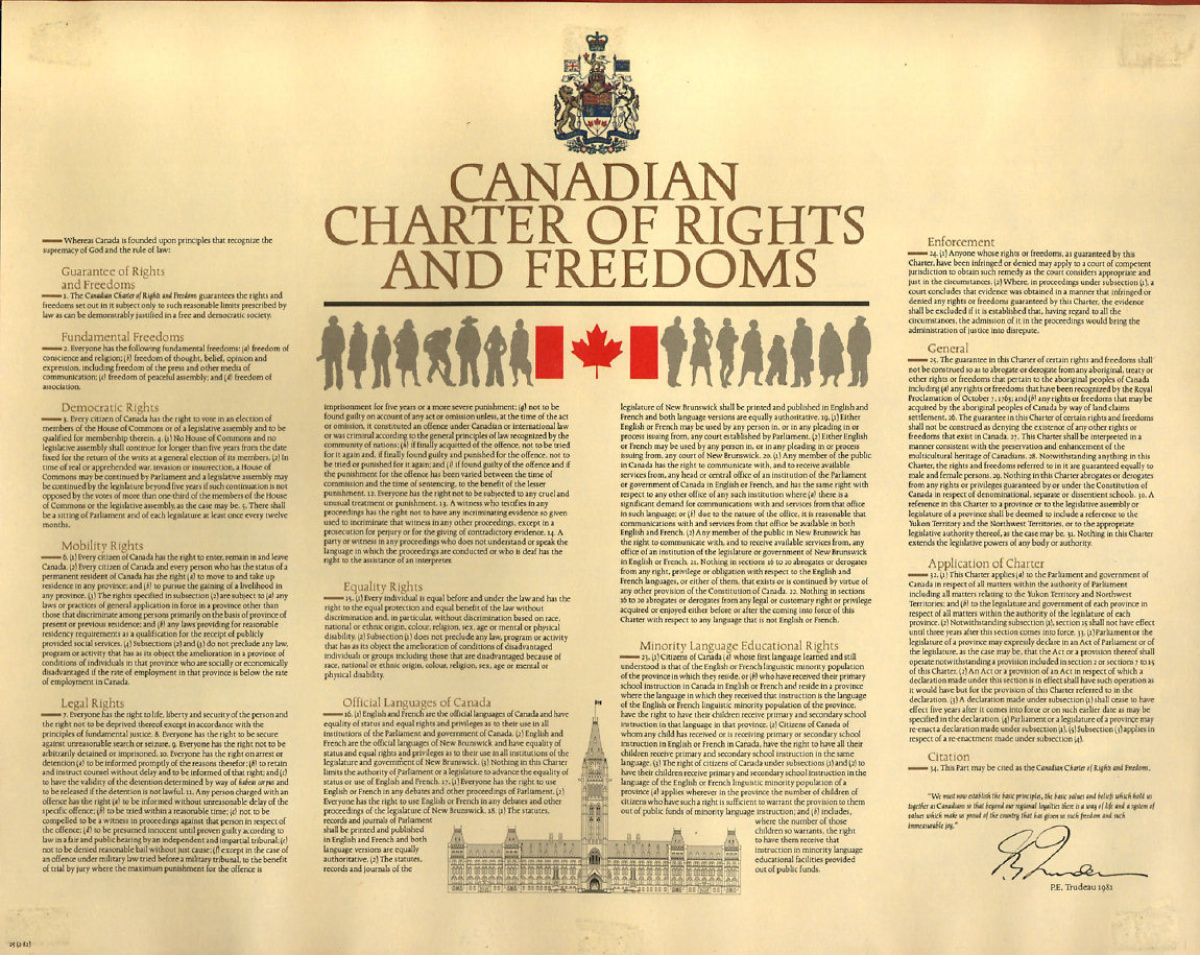
\includegraphics[width=0.85\textwidth]{images/charter.jpeg}
\end{center}

\end{frame}


\begin{frame}
\frametitle{The Charter of Rights and Freedoms}
The charter forms the first 34 sections of the Act.

\begin{itemize}
	\item Fundamental freedoms
	\item Democratic, mobility, legal and equality rights
	\item Official languages of Canada
	\item Minority language education rights
	\item Enforcement, general, and application
	\item It is also subject to the notwithstanding clause (s. 33)
\end{itemize}

\end{frame}



\begin{frame}
\frametitle{Guarantee of Freedoms}

The Charter begins with:

1. The Canadian Charter of Rights and Freedoms guarantees the rights and freedoms set out in it subject only to such reasonable limits prescribed by law as can be demonstrably justified in a free and democratic society. (Section 1).


\end{frame}



\begin{frame}
\frametitle{Guarantee of Freedoms}

In Regina v Oakes, 1986, Chief Justice Dickson developed the Oakes test for violations:  
\begin{enumerate}
\item There must be a pressing and substantial objective
\item The means must be proportional 
	\begin{enumerate}[a]
		\item The means must be rationally connected to the objective
		\item There must be minimal impairment of rights
		\item There must be proportionality between the infringement and objective
	\end{enumerate}
\end{enumerate}

\end{frame}



\begin{frame}
\frametitle{Fundamental Freedoms}

2. Everyone has the following fundamental freedoms:

\begin{enumerate}[a]
	\item freedom of conscience and religion;
	\item freedom of thought, belief, opinion and expression,
		including freedom of the press and other media of
		communication;
	\item freedom of peaceful assembly; and
	\item freedom of association
\end{enumerate}

\end{frame}



\begin{frame}
\frametitle{Democratic Rights}

3. Every citizen of Canada has the right to vote in an election of the members of the House of Commons or of a legislative assembly and to be qualified for membership therein 

4. (1) No House of Commons and no legislative assembly shall continue for longer than five years from the date fixed for the return of the writs at a general election of its members. (2) The war, invasion or insurrection exception...s

5. There shall be a sitting of Parliament and of each legislature at least once every twelve months.

\end{frame}



\begin{frame}
\frametitle{Mobility Rights}

The mobility rights include:

(1) Every citizen of Canada has the right to enter, remain in and leave Canada.\\
(2) Every citizen of Canada and every person who has the status of a permanent resident of Canada has the right
\begin{enumerate}[a]
 \item to move to and take up residence in any province; and
 \item  to pursue the gaining of a livelihood in any province. 
\end{enumerate}

\end{frame}



\begin{frame}
\frametitle{Legal Rights}

The legal rights include:

7. Everyone has the right to life, liberty and security of the person...

8. Everyone has the right to be secure against unreasonable search or seizure.

9. Everyone has the right not to be arbitrarily detained or imprisoned.

10. Everyone has the right on arrest or detention to be informed promptly of the reasons therefore, to retain and instruct counsel without delay and to be informed of that right, and the habeas corpus clause.

\end{frame}



\begin{frame}
\frametitle{Legal Rights}

11. Any person charged with an offence has the right to be informed of the specific offence, be tried within a reasonable time, not be compelled to be a witness, be presumed innocent, not be denied reasonable bail, be tried by a jury if the maximum punishment is five or more years, not be found guilty unless the action constituted an offence, not to be tried again, and receive a lesser punishment.

\end{frame}



\begin{frame}
\frametitle{Legal Rights}

12. Everyone has the right not to be subjected to any cruel and unusual treatment or punishment. 

13. A witness who testifies in any proceedings has the right not to have any incriminating evidence so given used to incriminate that witness in any other proceedings, ...

14. A party or witness in any proceedings who does not understand or speak the language in which the proceedings are conducted or who is deaf has the right to the assistance of an interpreter.

\end{frame}



\begin{frame}
\frametitle{Equality Rights}

The next section is a guarantee of equal rights:

15.	(1) Every individual is equal before and under the law and has 
	the right to the \textbf{equal protection and equal benefit} of the law
	without discrimination and, in particular, \textbf{without discrimination 
	based on race, national or ethnic origin, colour, religion, sex, age or mental or physical disability.}

(2) Subsection (1) does not preclude any law, program or 
	activity that has as its object the amelioration of conditions of 
	disadvantaged individuals or groups including those that are 
	disadvantaged because of race, national or ethnic origin, 
	colour, religion, sex, age or mental or physical disability.


\end{frame}



\begin{frame}
\frametitle{Remaining Sections}

	The next sections cover the official languages of Canada, minority language education rights, the enforcement of the Charter, and other general sections.
	
	Section 32 states that the charter only applies to the federal and provincial governments.
	
	It also gave some time for equality rights to come into effect.
	
\end{frame}



\begin{frame}
\frametitle{The Notwithstanding Clause}

Recognizing that there are very few rules that don't have exceptions, the authors included one in the charter.

This is known as the Notwithstanding Clause.

It is controversial and has been a subject for much debate over the years.

It allows the legislature to ignore certain provisions of the charter (!).

\end{frame}



\begin{frame}
\frametitle{The Notwithstanding Clause}

  (1) Parliament or the legislature of a province may expressly declare
	in an Act of Parliament or of the legislature that the Act or a provision 
	thereof shall operate notwithstanding a provision included in section 2 
	or sections 7 to 15.
  
	(2) An Act or a provision of an Act in respect of which a declaration 
	made under this section is in effect shall have such operation as it 
	would have but for the provision of this Charter referred to in the 
	declaration.
  
	(3) A declaration made under subsection (1) shall cease to have effect 
	five years after it comes into force or on such earlier date as may be 
	specified in the declaration.
  
		(4) Parliament or the legislature of a province may re-enact a 	declaration made under subsection (1).
  
		(5) Subsection (3) applies in respect of a re-enactment made under 
	subsection~(4).

\end{frame}



\begin{frame}
\frametitle{Or, in Plain Language}

Any Act of Parliament or of a legislature may violate the fundamental freedoms, the legal rights or the equality rights of Canadians... 

As long as the act expressly says it is doing so.

All other rights are inalienable.

If the next sitting of the legislature does not re-enact the declaration, then it is no longer in effect.

\end{frame}



\begin{frame}
\frametitle{But Why?!}

The charter is a written collection of rights in the Constitution Act, 1982.

The notwithstanding clause, however, protects the Supremacy of Parliament.

	In the words of Jean Chr\'etien, it prevents the Supreme Court from legalizing hate speech or child pornography as freedom of expression.

\end{frame}


\begin{frame}
\frametitle{Use of the Clause}

To date, the federal government has not used it.

The Alberta provincial government tried to use to prevent the legalization of same-sex marriage.\\
\quad But the Supreme Court found this law to be \textit{ultra vires}.

The Parti Qu\'eb\'ecosi used it in all of its laws in 1982.

Bill 101 (``The Charter of the French Language'') was found to be unconstitutional because it restricted freedom of expression.\\
\quad Bill 178 was used to insulate it from the charter.\\
\quad The law was later amended so as not to require the clause.

Saskatchewan included it, unnecessarily, in back-to-work legislation.

\end{frame}



\begin{frame}
\frametitle{Interpretation of the Charter}

The Supreme Court is the final interpreter of the Constitution and therefore the Charter.

If a law is ruled unconstitutional because it violates the charter, the only way to enact that law is to use the notwithstanding clause.


\end{frame}



\begin{frame}
\frametitle{The Supreme Court}

This is the second time we have mentioned the Supreme Court of Canada and its role in the legal system.

The Supreme Court receives a lot of attention, but most cases are resolved in lower courts.

Next, we will examine the Canadian Legal System in more detail.

\end{frame}

\begin{frame}
\frametitle{References \& Disclaimer}
\bibliographystyle{alphaurl}
\setbeamertemplate{bibliography item}{\insertbiblabel}
{\scriptsize
\bibliography{290}
}
\vfill

{\tiny Disclaimer: the material presented in these lectures slides is intended for use in the course ECE~290 at the University of Waterloo and should not be relied upon as legal advice. Any reliance on these course slides by any party for any other purpose are the responsibility of such parties.  The author(s) accept(s) no responsibility for damages, if any, suffered by any party as a result of decisions made or actions based on these course slides for any other purpose than that for which it was intended.\par}


\end{frame}


\end{document}

